\documentclass[sigconf]{acmart}

\copyrightyear{2017} 
\acmYear{2017} 
\setcopyright{acmcopyright}
\acmConference{ICMR '17}{}{June 6--9, 2017, Bucharest, Romania}
\acmPrice{15.00.}
\acmDOI{http://dx.doi.org/10.1145/XXXXXXX.XXXXXXX}
\acmISBN{ISBN 978-1-4503-4701-3/17/06} 
%Authors, replace the red X's with your assigned DOI string. See pdf attached to ACM rightsreview confirmation email.

\usepackage{booktabs} % For formal tables
\usepackage{algorithm}
\usepackage{multirow}
\usepackage{algorithmic}
\usepackage[bf, medium]{titlesec}

\DeclareMathOperator*{\argmax}{argmax}
\DeclareMathOperator*{\argmin}{argmin}
\renewcommand{\algorithmicrequire}{\textbf{input:}}
\renewcommand{\algorithmicensure}{\textbf{output:}}
% for saving space
\setlength{\abovecaptionskip}{1pt}
\setlength{\belowcaptionskip}{2pt}
\setlength{\intextsep}{1pt}
\setlength{\textfloatsep}{0pt}
\setlength{\floatsep}{1pt}
\setlength{\dbltextfloatsep}{1pt}
\setlength{\dblfloatsep}{1pt}
\titlespacing\section{0pt}{7pt minus 2pt}{0 pt plus 2pt}
\titlespacing\subsection{0pt}{7pt minus 2pt}{0pt plus 2pt} 
\titlespacing\subsubsection{0pt}{7pt minus 2pt}{0pt plus 2pt}


\begin{document}
\title{Joint Saliency Estimation and Matching using Image Regions for Geo-Localization of Online Video}

\author{Haoyue Shi}
\affiliation{
  \institution{School of EECS, Peking University}
  \streetaddress{No.5 Yiheyuan Rd.}
  \city{Beijing} 
  \country{P. R. China} 
  \postcode{100871}
}
\email{hyshi@pku.edu.cn}

\author{Jia Chen}
\affiliation{
  \institution{Language Technologies Institute, Carnegie Mellon University}
  \streetaddress{5000 Forbes Avenue}
  \city{Pittsburgh} 
  \state{PA}
  \country{USA} 
  \postcode{15213}
}
\email{jiac@cs.cmu.edu}


\author{Alexander G. Hauptmann}
\affiliation{
  \institution{Language Technologies Institute, Carnegie Mellon University}
  \streetaddress{5000 Forbes Avenue}
  \city{Pittsburgh} 
  \state{PA}
  \country{USA} 
  \postcode{15213}
}
\email{alex@cs.cmu.edu}
\renewcommand{\shorttitle}{JSEM using Image Regions for Geo-Localization for Online Video}


\begin{abstract}
In this paper, we study automatic geo-localization of online event videos, which is a key component behind various event analysis tasks such as cross-camera tracking and 3D reconstruction from co-located videos generated by multiple users. 
Different from general image localization task through matching, the appearance of an environment during significant events varies greatly from its daily appearance, since there are usually crowds, decorations, obstructions or even destruction when a major event happens. 
This introduces a major challenge: matching the event environment to the daily environment, e.g. as recorded by Google Street View. 
We observe that some regions in the image, as part of the environment, still preserve the daily appearance even though the whole image (environment) looks quite different. 
Based on this observation, we formulate the problem as joint saliency estimation and matching at the image region level, as opposed to the key point or whole-image level. 
As image-level labels of daily environment are easily generated with GPS information, we treat region based saliency estimation and matching as a weakly labeled learning problem over the training data. 
Our solution is to iteratively optimize saliency and the region-matching model. 
For saliency optimization, we derive a closed form solution, which has an intuitive explanation. 
For region matching model optimization, we use self-paced learning to learn from the pseudo labels generated by (sub-optimal) saliency values. 
In the test stage, we retrieve daily environment images for each frame in the video based on an image level similarity score calculated by region saliency and matching. 
We combine the GPS information of the retrieved and matched images to get the final geo-location for the video. 
We conduct extensive experiments on two challenging public datasets: Boston Marathon 2013 and Tokyo Time Machine. 
Experimental results show that our solution significantly improves over matching on whole images and the automatically learned saliency is a strong predictor of distinctive building areas. 
\end{abstract}

\keywords{Video Geo-Localization, Region Saliency, Region Matching}

\maketitle

\section{Introduction}
% task introduction
% jiac: I'm lazy and some of the content in this paragraph is almost the same as that in 1st paragraph in the technical report. Would you please slightly change the presentation of these sentences? Especially the 1st sentence. 
% it would be better to also ps different view images of the boston dataset in th figure~\ref{fig:library}
With the popularity of smartphones equipped with high quality cameras, events around the world can be quickly captured by videos and rapidly shared via social media.
When an event happens, different videos capture the same event at different positions from different perspectives.
For example, videos from surveillance cameras usually cover the event from a fixed location from 45 degree angle; 
videos from television reporters usually record the event in a rather professional perspective (helicopter view or first person view) at major locations; 
the videos from passersby usually capture event from a personal perspective at side locations that are often not covered by the news reporters.
On the one hand, knowing where is the video content is the basic and essential element behind various event analysis tasks such as person tracking and scene reconstruction. 
On the other hand, unlike EXIF meta-data in images, most of the videos shared online don't come with GPS information together. 

% task definition
In this paper, we study the problem of automatic event video localization. 
The input of event video localization is the query, event video, and the database, environment images with gps information, which could be street view images if the event video is taken on the ground or satelite images if the event video involves a 45 degree view. 
The task is to localize the event video by matching its content to the database. 
To be specific, event video and environment images belong to two different domains and it is actually a cross-domain matching problem.  
% original:
% Image geo-localization is a task which requires to use computer vision techniques to estimate the location (often GPS) of a given ground-level image by matching it to a reference database. 
% In their previous work, Hays and Efros~\cite{hays2008im2gps} have proved the feasibility of this task by leveraging over 6 million GPS-tagged images from the Internet.

% related work of retrieval in the same domain, point out the gap between the previous dataset and the real-word application
Abundant research works have been conducted in a related problem: general image localization through matching\cite{Arandjelovic_2013_CVPR}\cite{Arandjelovic16}\cite{hays2008im2gps} on public image datasets such as paris dataset\cite{philbin08lost} and oxford building\cite{philbin07object}.
Most of the query images in these datasets are photos of the landmarks in regular days. 
However, the appearance of the location could change a lot when an event happens. 
Here we give an example of location appearance change: Boston Marathon 2013 finish line explosion event. 
As shown in Figure~\ref{fig:library}, the appearance of the finish line was quite different from the regular day appearance: additional audience stands were added to the sidewalk and blue end banner was raised. 
When an event happens, e.g. parade, protest or attack, the appearance of the district is usually changed to some extent by either manual decoration or manual destruction. 
Thus, such dramatic appearance change is very common and not neglectable in event video localization task. 
To the best of our knowledge, the only public dataset that is built to take into account large appearance change is Tokyo Time Machine (TTM) dataset\cite{Arandjelovic16}.  
However, it only contains street view images taken in regular days while the variety of event videos are much large, including both 45 degree view and street view on event days. 
% original:
% There are already a lot of works focusing on the matching or image geo-localization task. 
% Universal Correspondence Network\cite{choy_nips16} is an efficient method to extract features from images and solve such image localization problems by matching, while requiring patch-level labelled instances for training. 
% Researchers have already released a lot of image-level labelled datasets. 
% However, to the best of our knowledge, there isn't any large-scale patch-level labelled dataset for the task of image localization. 
% What's more, NetVLAD~\cite{Arandjelovic16} proposed by Arandjelovic et al. is a nearly perfect method to solve the place recognition problem, which is very similar to image localization problem. 
% But we still wonder whether we could align the matching score to patch-level. 
% In other words, we aim to let the computer output the reason of why two images match or mismatch in patch-level, in order to further improve the performance for the image matching problem. 
% In addition, real world may change everyday, especially when some event happens. 
% To avoid the noise caused by daily events, we need some improvement on previous image localization/matching methods.

% problem formulation and its benefits
The major challenge of event video localization lies in cross-domain large appearance change. 
Instead of modeling it as a single learning to match problem, we formulate the task as a joint saliency detection and matching problem, which simultaneously outputs the matching score and the matched region as supporting evidence. 
Such problem formulation benefits us in three aspects.

First, by explicitly introducing saliency detection in the model, we are able to distinguish between meaningful matching and meaningless matching. 
For example, the matching between building areas across two images are meaningful as building ares are usually distinctible for localization. 
The matching between road and tree areas across two images are meaningless as such matching could occur in and is not helpful for localization. 
Saliency detection helps to distinguish between these two types of matching and its result will be used to downweight the meaningless matching and emphasize on meainingful matching in our joint model. 

Second, joint modeling preserves the interdepency between saliency detection and matching. 
Region saliency is actually domain dependent and depends to matching. 
For example, if a video frame region matches many irrelevant environment images district A , it is not reliable to localize the video in district A based on this frame region. 
That is, this video frame region is not salient in district A. 
Now consider the same video frame region but the environment images of a different district B. 
The same video frame region may only match a few relevant environment images in district B, which means that it is reliable to localize the video based on this frame region in district B. 
That is, the same video frame region turns to be salient in district B. 
In our solution, we capture such interdepency between saliency detection and matching. 

Third, addition output of matched region makes the system output more explainable. 
For example, when the system fails, the ``matched'' region will be shown users that there is not enough distinctable environment clues in the video content so that it fails reasonably. 
Given such supporting evidence, the users will be more likely to trust the system as they learn to know the capability limit of the system in their usage. 

% jiac: please add some brief explanation for the 1st and 2nd component
% I'll extend the 3rd component after completing the solution part modification. 
Our solution is composed of three components:\\*
1. automatic weak label generation. \\*
2. matching based data-driven saliency estimation\\*
3. self-paced learning for joint salient detection and matching\\*
% original:
% Thus, we propose a method to solve the problem of cross-domain (event domain and satellite image database domain) video geo-localization by matching with weakly labelled (image level labelled rather than patch-level labelled) data, while the matching procedure is guided by the saliency of patches. 
% In our method, the saliency of patches are estimated automatically without any further manual work.

% It's much easier for human beings to determine the geo-location for photographs of famous scenes rather than those of oceans, grasslands or even ordinary houses. 
% This is because the famous scenes are rare, so that they are more discernible than oceans, grasslands and ordinary houses.
 
% Similarly, buildings, especially famous buildings, are always more discernible than roads, trees, etc.  
% Figure~\ref{fig:library} is a photograph of Boston Public Library, McKim Building. When determining the geo-location of the image, we would focus on the discernible (salient) regions but not the non-salient ones, since only the former could provide us information about the location. 
% In Figure~\ref{fig:library}, regions in red frames are salient while those in blue frames are not.
\begin{figure}[htbp]
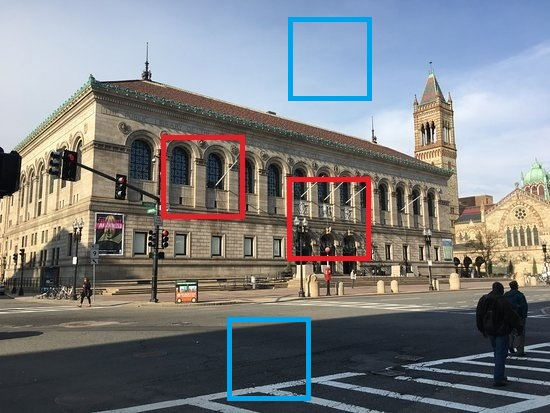
\includegraphics[width=0.41\textwidth]{img/library}
\\[0.1cm]
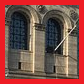
\includegraphics[width=0.1\textwidth]{img/library_1}

\includegraphics[width=0.1\textwidth]{img/library_2}

\includegraphics[width=0.1\textwidth]{img/library_3}

\includegraphics[width=0.1\textwidth]{img/library_4}
\caption{An example of salient regions and non-salient regions of an image.}
\label{fig:library}
\end{figure}

% too many details, may move to beginning of solution section
% Therefore, we aim to use the attribute of saliency to guide image/video localization. 
% To estimate how salient a region is, we reconsider the fact that non-salient regions are less discernible. 
% In other words, non-salient regions would be more common than salient ones in the database. We introduce the concept \textbf{saliency score} to measure how salient a region is. 
% An intuitive idea is to set saliency score of a region inversely proportional to the number of its similar regions in the database. 
% To evaluate how similar two regions are, we need to apply convolutional neural network (CNN), which has been widely used in the field of deep learning, to extract features from images. 

% In another hand, after estimating the saliency score of each region in an image. 
% We propose an attention-based model to guide the geo-localization system to pay more attention to salient regions when localizing an image. 
% Consequently, the model tends to be a joint model to both estimate saliency score of regions utilizing a matching model and optimize the matching model with the saliency score. 

% We evaluate our method on two video/image geo-localization datasets. 
% The experimental result on Boston dataset have shown that our method works well on event video frame geo-localization task. 
% We also evaluated it on the Tokyo Time Machine dataset~\cite{Arandjelovic16} in order to support the efficiency of our method.

The contributions of this paper are threefold. 
\begin{enumerate}
\item We formulate the event video localization task as a joint saliency detection and matching problem. 
Such formulation distinguishs between meaningful matching and meaningless matching adaptively to district domain, preserves the interdependency between saliency and matching and enhances system explainability.  
\item We propose a self-paced learning styled solution for the joint model, which starts from easy saliency detection and matching cases and gradually move on to hard saliency detection and matching cases. 
% \item We demonstrate that saliency is an effective attribute to guide image/video localization. 
% \item We propose a method which can joint estimate the saliency score of image regions and geo-localize an image or a video.
% \item Our method is helpful for real world event related video geo-localization and it is efficient to solve cross-domain matching problems.
\end{enumerate}

% section arrangement
The rest of the paper is organized as follows. 
Section~\ref{sec:related} introduces related work. 
Section~\ref{sec:problem} formalizes the problem for the video event localization task. 
Section~\ref{sec:solution} gives the solution to the problem. 
Section~\ref{sec:expr} presents the experiment results. 
Section~\ref{sec:conclusion} draws some conclusions. 

\section{Related Work}
\label{sec:related}
%video/image geo-localization
As we have mentioned in Section~\ref{sec:introduction}, early work by Hays and Efros~\cite{hays2008im2gps} revealed the feasibility of the image localization task. % this work doesn't make sense at all. don't give too much credit to it. 
Zamir and Roshan~\cite{zamir2010accurate} used SIFT descriptors for image localization by voting, and constructed a dataset based on Google Street-View to test the efficiency of the algorithm. 
Lin et al.~\cite{lin2013cross} proposed the first ground-to-overhead geo-localization method, of which the key idea is to learn the relationship between the ground-level images and their over-head appearances. 
After that, Lin et al.~\cite{lin2015learning} then published an approach by convolutional neural network(CNN) to learn deep representations for ground-to-overhead geo-localization. 
Vo and Hays~\cite{vo2016localizing} then explored several deep CNN architectures for the cross-domain matching and improved the accuracy of image geo-localization. 
What's more, Bansal et al.~\cite{bansal2012ultra} proposed a method to capture the structure of self-similarity of patterns on facades for image geo-localization.

Leung et al.~\cite{leung2008localization} designed a monocular vision based particle filter localization system for urban settings that uses aerial reference map. 
However, because of the great similarity between the task of image localization and video localization, researchers often treat them as the same task.

Visual place recognition is a similar task of image geo-localization. 
Arandjelovic et al.~\cite{Arandjelovic16} developed NetVLAD, a CNN architecture of which the main component is the VLAD (``Vectors of Locally Aggregated Descriptors'') layer and got the state-of-the-art performance on two challenging place recognition datasets. 

While attention-based models are widely used in recognition tasks, many recent works show that attention-based model can improve the performance of machine learning models~\cite{mnih2014recurrent,zheng2015neural}. 
The key idea of attention-based model is to add attention information to build a representation. 
This idea is intuitive. 
For example, when looking at an image, we human beings often recognize the objects on it and then receive the information from the background, rather than receiving information simultaneously from the foreground objects and background scenes. 
In our approach, we compute the attention to each region by its saliency. 

% self-paced learning
In machine learning, a sequence of gradually  added training samples~\cite{bengio2009curriculum} is called a curriculum. 
Inspired by the cognitive process of humans and animals, a straightforward way to generate such a sequence is to add samples based on their ``easiness" to learn. 
However, such ``easiness" is based on specific problem and hard to generalize. 
In order to solve this problem, Self-Paced Learning (SPL) was introduced by Kumar et al.~\cite{kumar2010self}, which embeds curriculum designing into model learning. 
In SPL, the curriculum is gradually generated by the model itself based on what it has learned, and it's also a general implementation for curriculum learning. 
Following that, several works have improved self-paced learning~\cite{jiang2014easy,tang2012shifting,jiang2015self}. 
In this paper, we propose self-paced learning method to automatically estimate the saliency score for each region of a frame.


\section{Problem Formulation}
\label{sec:problem}
The event video localization task is to retrieve environment images from database given the query event video. 
The database images are automatically downloaded from online map service given a circle or rectangle shaped district where the event happened. 
If the video is taken on the ground, the database images will be Google street view images;
if the video is taken from a 45 degree up to down perspective of view, the database images will be Google satellite images. 
The details of database image generation will be elaborated in section~\ref{sec:solution}. 

A query video is composed of frames $\{q\}$. 
As we process one frame per time in matching the database, we abbreviate one frame from the query video as query for the ease of representation. 
The environment image from the database is denoted as $d$ and the database is denoted as $D = \{d\}$. 
We divide images to different regions on multi-scales and each region is assigned a saliency score $s$ to indicate how import the region is in matching.  
We use subscript to represent region index. 
That is, we have saliency score $s(q_i)$ for region $i$ in query $q$ and $s(d_j)$ for region $j$ in the database image $d$. 
We define the non-negative matching score between two regions as $m(q_i, d_j; \mathbf{\Theta})$, where $\mathbf{\Theta}$ is the parameters to be learn. The similarity of two regions is proportional to their matching score.
For the ease of notation, we will use $m(q_i, d_j; \mathbf{\Theta})$ and $m(q_i, d_j)$ interchangeably in the following. 

Now we have defined regions in the image, saliency score on regions and matching score between regions. 
Putting all these together, we define the matching score between query and database image as weighted sum of region matching scores:
\begin{align}
\label{eq:img_match}
M(q, d) &= \sum_{i, j} w_{ij} m(q_i, d_j)\\
\label{eq:weight}
w_{ij} &= s(q_i) + s(d_j)
\end{align}
where the weight $w_{ij}$ is defined as the sum of saliency score of both regions. 
On the one hand, if both regions are salient and their matching score is high, such region pair contribute much to the final matching score $M(q, d)$. 
On the other hand, even if the matching score between two regions is high, but if both regions are not salient (e.g. road or tree), such region pair doesn't contribute much to the final matching score $M(q, d)$. 
% In the test stage, we assign the location of the query by averaging GPS location of top $K$ retrieved environment images. 

In the training stage, we automatically generate the labels of image pairs from database $D$ by leveraging the GPS information assigned to each environment image. 
The label $y_{(q, d)}$ of image $q$ and $d$ is $1$ if two images are matched and $0$ vice versa. 
The training data is denoted as: 
\begin{align}
D_{train} &= \{(q, d, y_{(q, d)})\}\\
q &\in D \nonumber \\
d &\in D \nonumber
\end{align}
The details of automatically generating $D_{train}$ from $D$ are given in section~\ref{sec:solution}. 
Note that the labels are given on image pairs rather than region pairs. 
As the matching model $m(q_i, d_j; \mathbf{\Theta})$ is defined on region pair, the labels are actually weak labels. 
We use contrastive noise loss function as $L(q, d, y)$:
\begin{equation}
\label{eq:img_loss}
\begin{aligned}
L(q, d, y) &= y\, L_P(q, d, y) + (1-y)\, L_N(q, d, y) \\
L_P(q, d, y) &= -\sum_{y_{(q, d)}=1} M(q, d)\\
L_N(q, d, y) &= -\sum_{y_{(q, d)}=0} \max(0, \Delta-M(q,d))
\end{aligned}
\end{equation}
where $\Delta$ is a hyper-parameter to keep unmatched pairs having small matching scores, $L_P$ is the loss function for matched pairs, $L_N$ is the loss function for unmatched pairs. 
We use eq~\eqref{eq:img_match} to expand image matching $M(q, d)$ term in the loss function: 
\begin{equation}
\label{eq:correspondence}
\begin{aligned}
L(q, d, y) = &-y\sum_{y_{(q, d)}=1} M(q, d) - (1-y) \sum_{y_{(q, d)}=0} \max(0, \Delta - M(q, d))\\
= & -y\, \sum_{i, j}\sum_{y_{(q, d)}=1} w_{ij}\, m(q_i, d_j) \\
 &- (1-y)\, \sum_{i, j}\sum_{y_{(q, d)}=0} w_{ij}\, \max(0, \Delta^{'} - m(q_i, d_j))\\
= & y\, \underbrace{\sum_{i, j} w_{ij}\, L_P(q_i, d_j)}_{L_P(q, d)} + (1-y)\, \underbrace{\sum_{i,j} w_{ij}\, L_N(q_i, d_j)}_{L_N(q, d)}
\end{aligned}
\end{equation}

In the last step substitution, we denote
\begin{equation}
\label{eq:region_loss}
\begin{aligned}
L_P(q_i, d_j, y) &= -\sum_{i,j}\sum_{y_{(q, d)}=1} m(q_i, d_j)\\
L_N(q_i, d_j, y) &= -\sum_{i,j}\sum_{y_{(q, d)}=0} \max(0, \Delta^{'} - m(q_i, d_j))
\end{aligned}
\end{equation}

The last step in eq~\eqref{eq:correspondence} shows that the two components in image level loss, $L_P(q, d, y)$ and $L_N(q, d, y)$, are weighted sum of the two components in region level loss, $L_P(q_i, d_j, y)$ and $L_N(q_i, d_j, y)$, respectively. 
Furthermore, if we consider the region level label to be the same as its corresponding image level label, i.e. $y_{(q_i, d_j)} = y_{(q, d)}$, we could see that region level loss $L_P(q_i, d_j, y)$, $L_N(q_i, d_j, y)$ in eq~\eqref{eq:region_loss} has exactly the same form of image level loss $L_P(q, d, y)$, $L_N(q, d, y)$ in eq~\eqref{eq:img_loss}. 
However, recall that the major challenge in event video localization, large appearance change, leads to the fact that $y_{(q,d)} = 1$ doesn't imply that $y_{(q_i, d_j)} = 1, \forall q_i \in q, \forall d_j \in d$. 
In our problem formulation, we solve this issue by multiplying a region pair dependent weight $w_{ij}$ to each region level loss $L_P(q_i, d_j)$. 
Note that $w_{ij}$ is defined by saliency $s(q_i)$ and $s(d_j)$. 
That is, we could suppress the influence of ``wrong'' region level label to the final loss function through saliency. 

We recap all the above deduction into one main problem. 
\begin{equation*}
\begin{aligned}
\text{main problem:}\\
min_{\mathbf{S}, \mathbf{\Theta}} L(q, d, y; \mathbf{S}, \mathbf{\Theta}) &= -y\, \sum_{i, j}\sum_{y_{(q, d)}=1} w_{ij}\, m(q_i, d_j; \mathbf{\Theta}) \\
& - (1-y)\, \sum_{i, j}\sum_{y_{(q, d)}=0} w_{ij}\, \max(\Delta^{'}-m(q_i, d_j; \mathbf{\Theta}))\\
w_{ij} &= s(q_i) + s(d_j)\\
\mathbf{S} &= \{s(q_i)\} \cup \{s(d_j)\}\\  
s.t. & ||s(q)||_2 = 1 \quad \forall q\\
& ||s(d)||_2 = 1 \quad \forall d\\
& s(q_i), s(d_j) \in [0,1] \\
& y\in \{+1, 0\}
\end{aligned}
\end{equation*}
The notations introduced in this section are summarized in table~\ref{table:notations}. 

\begin{table}[htbp]
\begin{center}
\begin{tabular}{|c|p{0.35\textwidth}|}
\hline
$q_i$ & region $i$ in the query image $q$\\[0.2cm]
$d_j$ & region $j$ in the database image $d$\\[0.2cm]
$s(q_i), s(d_j)$ & the saliency of the region $q_i, d_j$ \\[0.2cm]
$m(q_i, d_j)$ & non-negative matching score between region $q_i$ and $d_j$ \\[0.2cm]
$Q$ & all video frames $\{q\}$ \\[0.2cm]
$D$ & all database images $\{d\}$ \\[0.2cm]
\hline
\end{tabular}
\end{center}
\caption{Notations introduced in this section.}
\label{table:notations}
\end{table}

\section{Solution}
\label{sec:solution}
\subsection{Training}
The main problem is non-convex and very difficult to optimize. 
One typical solution is to use cyclic coordinate method (CCM)\cite{GorskiPK07}. 
To be specific, we iteratively optimize the objective function by fixing $\mathbf{S}$ with respect to $\mathbf{\Theta}$ and vice versa. 
The major problem in such approach is that the quality of the solution depends highly on the initialization as it converges to a local minimum. 
To be specific, if we get a good estimation of $\mathbf{S}$, it is relatively easy to get a good solution for $\mathbf{\Theta}$ as the final loss function puts more emphasis on the correct region pair matching and vice versa. 

Thus, we propose a region based joint model on saliency estimation and region matching for training. Our pipeline is composed of five main steps: 

1.	\emph{Image level (weak) label generation.} 
In this step, we generate the weak labels based on GPS information automatically. 
Google Map provides satellite images, as well as street view images, together with their GPS information to users, so that we can download them conveniently as database. 
Figure~\ref{fig:dbregion} (color masked) shows the region that our database for Boston dataset (introduced in Section~\ref{sec:expr}) covers. 
The colored masks are drawn by Google Map automatically, indicating the buildings. 
\begin{figure}[t]
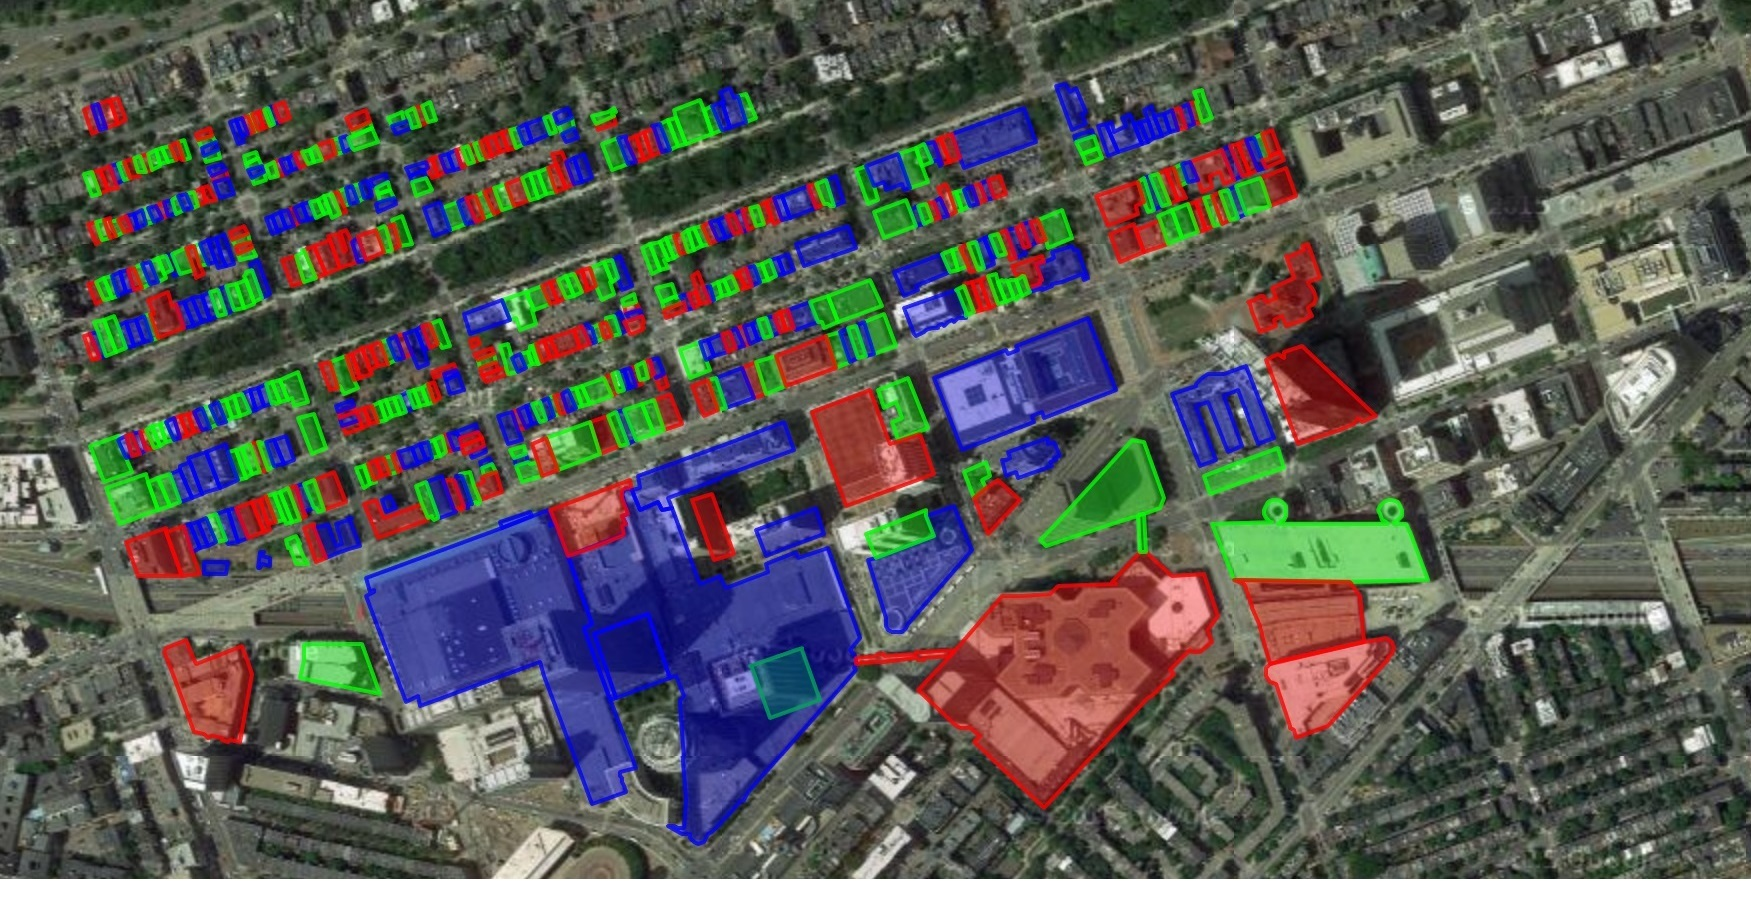
\includegraphics[width=0.7\linewidth]{img/db_region}
\caption{An example for collecting training data with Google Map.}
\label{fig:dbregion}
\end{figure}
After the generation of our database, we sample images in the range that the database covers randomly. 
Google Map provides four different perspectives of view from each point. 
If we just move the sampling point a little, the image with the same perspective would not change a lot. 
Thus, we can get two different images containing almost the same scene, and that is the rationality of our method to generate weak labels automatically.
More specifically, we use Euclidean distance to judge whether two sampling points are near to each other. 
We set the matching label of two images $q, d$ using 
\begin{equation}
\label{eq:weaklabel}
y_{(q, d)} = \left\{
\begin{aligned}
1 \qquad & dist(q,d) \leq \theta \\
0 \qquad & dist(q,d) > \theta
\end{aligned}
\right.
\end{equation}
where $q$ is the sampled image, $d$ is the image from our database, $dist(q,d)$ is the Euclidean distance between the locations of $q$ and $d$ in the real world, $\theta$ is a hyper-parameter that denotes the distance threshold of matching. 
In addition, by zooming, rotating and shifting, we can augment our database to let it contain images with larger diversity. 
Thus, we have completed the generation of training data $D_{train}$.
For database generation, we set $\theta = 25m$.\\[-0.25cm]

2. \emph{Initialization of matching model.}
In this step, we choose a good initialization of matching model. 
To be specific, we train a matching model $m(q_i, d_j; \mathbf{\Theta})$ directly using the image pairs. 
The structure of the network should be the same as that in the following procedure.
That is, we start from the degenerate case where the entire image is treated as one region.

In our training procedure, we applied Siamese network for initializing the matching model. 
The structure of the Siamese network we applied is shown in Figure~\ref{fig:siamese}.
The CNN is used to extract features from images. 
In this step, the region pairs are exactly image pairs themselves. 
We will introduce more details about the structure of the network in \emph{Step 4}.
\begin{figure}[htbp]
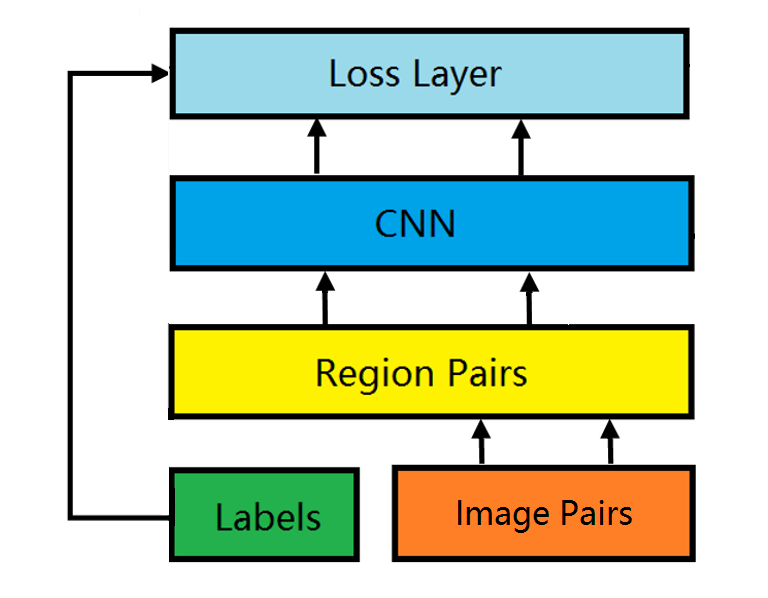
\includegraphics[width=0.6\linewidth]{img/siamese}
\caption{The structure of Siamese network. }
\label{fig:siamese}
\end{figure}

3. \emph{Saliency Estimation}. Apply the matching model $m(q_i, d_j; \mathbf{\Theta})$ on regions and optimize the main problem with respect to saliency $\mathbf{S}$. This problem can be decomposed to $|Q|+|D|$ separate linear objective quadratic constraint convex optimization problems:
\begin{equation}
\label{eq:decomposed_problem}
\begin{aligned}
& \max_{\mathbf{s}(q)} \sum_{q_i \in q} (m_{i\cdot}^+ - m_{i\cdot}^-) s(q_i) \\
\text{where} \\
m_{i\cdot}^+& = \sum_{\{d_j|y(q_i,d_j)=1\}} m(q_i,d_j) \\
m_{i\cdot}^-&=\sum_{\{d_j|y(q_i,d_j)=0\}} \min(0, m(q_i,d_j)-\Delta^{'})\\
s.t.& ||\mathbf{s}(q)||_2 = 1\\
& s(q_i)\in [0,1]
\end{aligned}
\end{equation}
We can add the other $|D|$ formulas with respect to $d$ analogously.
This problem has closed form solution:
\begin{equation}
\label{eq:closed_form_solution}
\begin{aligned}
& \mathbf{m}_q = [..., m_{i\cdot }^+ - m_{i\cdot}^-, ...] \geq \mathbf{0} \\
& \hat{\mathbf{s}}(q) = \frac{\mathbf{m}_q}{||\mathbf{m_q}||_2}
\end{aligned}
\end{equation}
Here, $m_{i\cdot }^+, m_{i\cdot}^-$ correspond to the matching status of $q_i$ to regions in positive labels and those in negative labels. 
Note that $m(q_i, d_j)$ is always non-negative due to our constraint in the section of problem formulation, $m_{i\cdot }^+$ is always non-negative and $m_{i\cdot }^-$ is always non-positive. Hence, we have the solution vector  $ \mathbf{m}_q = [..., m_{i\cdot }^+ - m_{i\cdot}^-, ...] \geq \mathbf{0} $. Analogously, we can compute the solution for $\hat{\mathbf{s}}(d)$.

The solution saliency $\hat{\mathbf{S}} = \{\hat{\mathbf{s}}(q)\} \cup \{\hat{\mathbf{s}}(d)\}$ can be used to generate pseudo labels on region level. 
The label is called ``pseudo'' because we fix the parameter $\mathbf{\Theta}$ from an imperfect matching model $m(q_i, d_j; \mathbf{\Theta})$ to get the solution. 

With the hypothesis that different parts of a building would not look very different, if an image pair $(q,d)$ is labelled as matched, then the pair of salient regions $(q_i, d_j)$ with high $s(q_i)$ and $s(d_j)$ should be matched with high level confidence. 
Oppositely,  if an image pair $(q,d)$ is labelled as unmatched, the pair of salient regions $(q_i, d_j)$ with high $s(q_i)$ and $s(d_j)$ should be unmatched with high level confidence, too. 
Thus, we use Eq~\eqref{eq:weight} (i.e. the sum of $s(q_i)$ and $s(d_j)$) to measure the confidence of the pseudo label $y_{(q,d)}$ for region pair $(q_i, d_j)$.

4. \emph{Region based matching optimization}. After estimating the saliency score of each region, we only use most confident pseudo region level labels to train the region matching model $m(q_i, d_j; \mathbf{\Theta})$. 
To refine the region level matching model, we minimize Eq~\eqref{eq:region_loss} as the loss function with the Siamese network structure, which has been shown in Figure~\ref{fig:siamese}. 
Since the training samples are fed to the network one by one (or batch by batch), the loss function for a region pair $(q_i, d_j)$ with label $y$ should be rewritten as 
\begin{equation}
L(q_i, d_j, y) = y\cdot m(q_i, d_j) + (1-y)\cdot \max(0, \Delta^{'} - m(q_i,d_j))
\label{eq:region_loss_sum}
\end{equation} 
where $\Delta^{'}$ is the hyper-parameter to keep unmatched pairs having a small matching score. 

5. We repeat step 3 and step 4 and gradually lower the confidence level for the pseudo label as the model becomes more and more accurate and we could rely on more pseudo labels generated. 
The confidence lowering procedure is controlled by the self-paced function\cite{jiang2015self}. 

In self-paced curriculum learning, a the self-paced function $f(\mathbf{v};\lambda)$ determines a learning scheme, where $\mathbf{v}\in [0,1]^n$ denotes a vector of weight variable for each training sample and $\lambda$ controls the learning pace. 
In a self-paced function, $||\mathbf{v}||_1$ increases with respect to $\lambda$. For a fixed function $f(\mathbf{v};\lambda)$, the sample selecting weight $\mathbf{v}$ can be computed by
\begin{equation}
\mathbf{v} = \argmin_{\mathbf{v}\in [0,1]^n}\sum v_il_i + f(\mathbf{v};\lambda)
\end{equation}
where $l_i$ is the loss function for the $i^{th}$ sample. 

To be more specific, we select training samples $\{(q_i, d_j, y)\}$by 
\begin{equation}
\mathbf{v} = \argmin_{\mathbf{v}\in [0,1]^n}\sum v_{ij}\frac{1}{s(q_i) + s(d_j)} + f(\mathbf{v};\lambda)
\label{eq:sample_selection}
\end{equation}
where $n$ denotes the total number of our candidate samples $(q_i, d_j, y)$. To make the loss function $l_i$ satisfy the requirements of self-paced learning scheme~\cite{jiang2015self}, we set $l_i = \frac{1}{s(q_i) + s(d_j)} $, which is the multiplicative inverse of Eq~\eqref{eq:weight}.

The self-paced function we apply is 
\begin{equation}
f(\mathbf{v};\lambda) = \lambda-||\mathbf{v}||_1 = -\lambda\sum_{i=1}^n v_i
\end{equation}
representing a linear scheme. 

Thus, we reformulate \emph{main problem} into a self-paced version. 

\text{self-paced version of main problem:}
\begin{equation*}
\begin{aligned}
min_{\mathbf{S}, \mathbf{\Theta}} L(q, d, y; \mathbf{S}, \mathbf{\Theta}) &= -y\, \sum_{i, j}\sum_{y_{(q, d)}=1} w_{ij}\, m(q_i, d_j; \mathbf{\Theta}) \\
& - (1-y)\, \sum_{i, j}\sum_{y_{(q, d)}=0} w_{ij}\, \max(\Delta^{'}-m(q_i, d_j; \mathbf{\Theta}))\\
& + f(w_{ij}; \lambda) \\
w_{ij} &= s(q_i) + s(d_j)\\
\mathbf{S} &= \{s(q_i)\} \cup \{s(d_j)\}\\  
f(w_{ij}; \lambda) &= \lambda - ||w_{ij}||_1 \\
s.t. & ||s(q)||_2 = 1 \quad \forall q\\
& ||s(d)||_2 = 1 \quad \forall d\\
& s(q_i), s(d_j) \in [0,1] \\
& y\in \{+1, 0\}
\end{aligned}
\end{equation*}
where $\lambda$ is a hyper-parameter to control the pace of learning in the self-paced procedure. 

In summary, our method can be described as Algorithm~\ref{alg:solution}.
\begin{algorithm}
\begin{algorithmic}[1]  
\REQUIRE{training dataset $D_{train}$, pre-trained matching model parameters $\mathbf{\Theta}$, self-paced function $f$ and stepsize $\mu$}\\
\ENSURE{saliency score $\mathbf{S}$ and refined matching parameters $\mathbf{\Theta^*}$ \\}
~\\
\STATE{Initialize $\mathbf{S}$, $\lambda$ and the matching model $\mathbf{\Theta^* = \Theta}$}
\WHILE{{\sl not converged}}
  \STATE{Estimate saliency score with Eq~\eqref{eq:closed_form_solution}}
  \STATE{Generate region level pseudo labels using image level labels}
  \STATE{Select ``easy'' samples by Eq~\eqref{eq:sample_selection}}
  \STATE{Refine $\mathbf{\Theta^*}$ with the loss function Eq~\eqref{eq:region_loss_sum}}
  \STATE{\textbf{if} $\lambda$ is small \textbf{then} increase $\lambda$ by $\mu$}
\ENDWHILE
\STATE{\textbf{return} $\mathbf{S}$, $\mathbf{\Theta^*}$}
\end{algorithmic}
\caption{Joint Saliency Estimation and Matching Optimization}
\label{alg:solution}
\end{algorithm}

\subsection{Inference}
After refining the matching model, we propose a corresponding region-based metric to measure the similarity between two images $q$ and $d$, which is 
\begin{equation}
sim_R(q,d) = -\sum_{q_i \in q} \min_{d_j\in d} \frac{|q_i|}{|q|} w_{ij}||f(q_i)-f(d_j)||_2
\label{eq:simR}
\end{equation}
where $|q_i|$ and $|q|$ is the size of region $q_i$ and image $q$, $f(q)$ and $f(d)$ are the vector representations of the two images in the feature space. 

Our method of video geo-localization is based on such fact: if a video has not been edited, the geo-location of it should not vary a lot in a short time. 
To find the geo-location of a video, we first retrieve $K$ most similar images in the database for each frame, and collect $K\times F$ images (may overlap) in the database. 
Then, we cluster the images in the database into $C$ clusters, based on their representative vectors in the feature space. 
The video will be localized to the average GPS coordinate of the largest cluster.

\section{Experiments}
\label{sec:expr}

In this section, we first give introduction to the two datasets we used to test our model; 
and then introduced the details in our implementation in experiments; 
next, we briefly introduce the evaluation metrics and baseline we applied.
We report the experimental results on joint model based geo-localization and saliency estimation in the last two sub-sections, and give some analysis.

\subsection{Datasets}
We use two challenging datasets, Boston Marathon 2013\cite{chen2016boston} and Tokyo Time Machine~\cite{Arandjelovic16}. 
Table ~\ref{table:dataset} shows the summary of the two datasets we used.
\subsubsection{Boston Dataset} 
~Chen et al.~\cite{chen2016boston} collected video clips which are related to the event of Boston Marathon bombing from the internet. 
This is a dataset which focus on a real event. 
In the videos, the streets look very different from daily appearance due to the event.
Figure~\ref{fig:bostonvideo} shows some example videos. 
In this dataset, they also provide $10,000$ satellite environment images in the surrounding region of the event location. 
The region contains $562$ buildings in total. 
We uniformly sampled 2,500 GPS locations in this region. 
For each GPS coordinate, we collected 4 images from 4 different perspectives of view (10,000 images in total).
We also collected the same number of images as queries for training at randomly sampled GPS locations in the same way to collect database.
For testing, we labeled the ground truth of geo-location for $100$ sampled frames from $37$ 45-degree-view video clips. Some example frames are shown in Figure~\ref{fig:bostonvideo}. Each frame may have multiple relevant images in the database.
\begin{figure}[htbp]
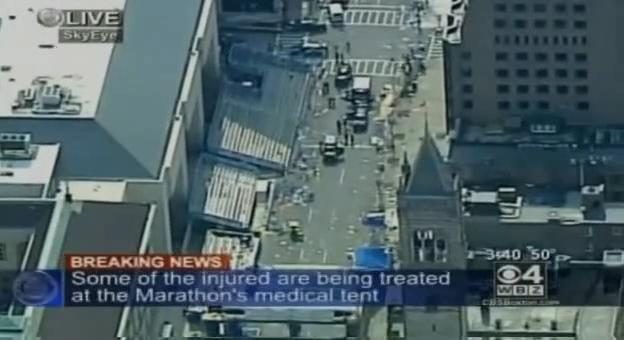
\includegraphics[width=0.4\linewidth]{img/video_1}
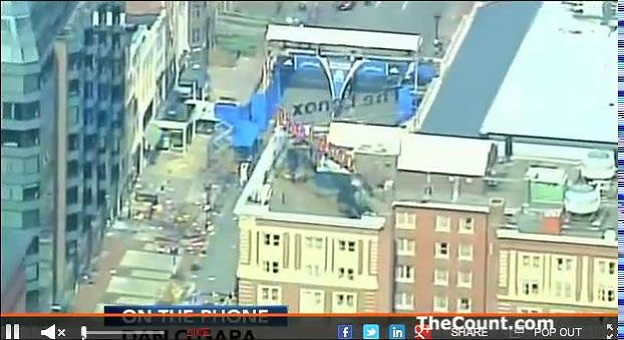
\includegraphics[width=0.4\linewidth]{img/video_2}
\\[0.1cm]
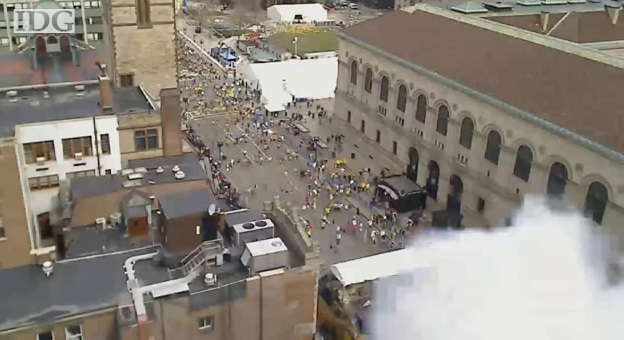
\includegraphics[width=0.4\linewidth]{img/video_3}
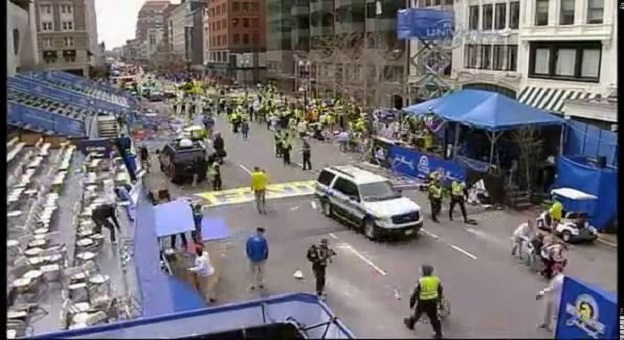
\includegraphics[width=0.4\linewidth]{img/video_4}
\caption{Sample video clips collected from the internet.}
\label{fig:bostonvideo}
\end{figure}


\subsubsection{Tokyo Time Machine Dataset} 
~Tokyo Time Machine (TokyoTM) dataset was released by Arandjelovic et al.~\cite{Arandjelovic16}, generated  from  downloaded  Time  Machine  panoramas. 
In this dataset, the appearances of buildings also change a lot, since the pictures were taken at different time in different days.

\begin{table}[htbp]
\begin{tabular}{l|rr}
Dataset & Database & Query set \\
\hline
\hline
Tokyo Time Machine-train & 49,104 & 7,277 \\
Tokyo Time Machine-val & 49,056 & 7,186 \\
Tokyo 24/7 (-test) & 75,984 & 1,125\\
\hline
Boston-train & 8,000 & 8,000 \\
Boston-val & 2,000 & 2,000 \\
Boston-test & 10,000 & 37 video clips
\end{tabular}
\caption{The size of the dataset we used in the experiments. The train/val(idation)/test dataset is mutually disjoint geographically.}
\label{table:dataset}
\end{table}


\subsection{Implementation Details}
In the following experiments, we use Caffe~\cite{jia2014caffe} as the deep learning framework.

We divide an image into a ``pyramid'', where the first layer is the image itself, the second layer contains $2 \times 2$ sub-images and the third layer contains $3 \times 3$ sub-images. 
Thus, each image has 14 regions when we apply our saliency guided geo-localization method. The saliency score of each region is estimated separately. 
Figure~\ref{fig:regions} shows how we generate regions for an image in the experiments. 

\begin{figure}[htbp]
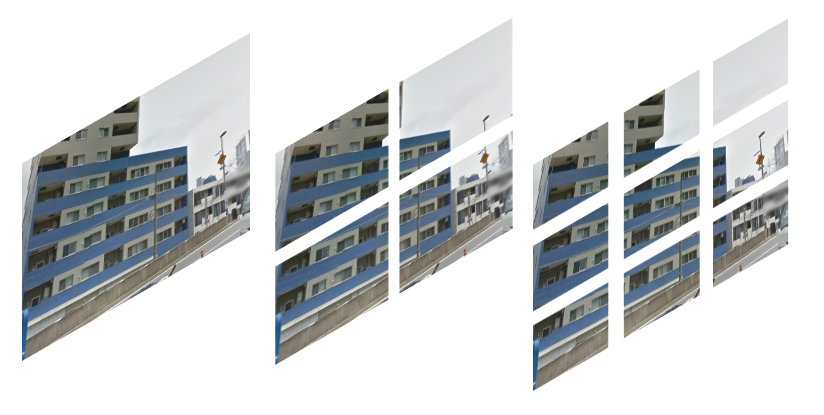
\includegraphics[width=0.8\linewidth]{img/regions}
\caption{The regions of an image in our experiments.}
\label{fig:regions}
\end{figure}

To compare with Eq~\eqref{eq:simR}, we also report the experimental results with another metric of similarity
\begin{equation} 
sim(q, d) =  -||f(q) - f(d)||_2
\label{eq:sim}
\end{equation}
which is directly the additional inverse of the Euclidean distance between two representative vectors in the feature space. 

\subsection{Evaluation Metrics and Baselines}
We test the performance of our model with adopting two common metrics: mean average precision (MAP) and recall on top$N$:\\
1. \emph{MAP} For a query image, the average precision of an image retrieval task can be computed by $AveP=\frac{\sum_{k=1}^nP(k)\times rel(k)}{number~of~relevant~images}$, where $P(k)$ is the precision at cut-off $k$ in the list; $rel(k)$ is an indicator function equalling $1$ if the image at rank $k$ is a relevant image, $0$ otherwise. Then $MAP=\frac{\sum_{i=1}^{|Q|}AveP(i)}{|Q|}$, where $|Q|$ is the number of queries. This metric shows the general performance for a model. \\
2. \emph{Recall on Top $N$.} We retrieve $N$ most similar images for each query. Therefore $Recall on top N = \frac{\sum_{i=1}^{|Q|} \#RetrievedRelevantImage(i)}{\sum_{i=1}^{|Q|} \# RelevantImage(i)}$, where $\#$ represents number. This metric is helpful to reveal the application value for a method, since we often retrieve top $N$ images for image retrieval tasks, like geo-localization.

We applied our method introduced in Section~\ref{sec:solution} with VGG-CNN-M model as a base CNN model and we introduce the following baselines:
\begin{itemize}
\item VGG-CNN-M-$sim$: it calculates similarity $sim$ by Eq~\eqref{eq:sim} using the $fc7$ layer output of the model released by Chatfield et al.~\cite{chatfield2014return}. 
\item VGG-CNN-M-$sim_R$: it estimates the saliency score using the VGG-CNN-M model, and then compute the similarity between image $q$ and $d$ by Eq~\eqref{eq:simR}. 
\item IBFT-$sim$: it applies image-level based fine-tuning to the matching model, and use Eq~\eqref{eq:sim} as the metric of similarity. 
\item JSEM-$sim_R$: it is the full joint saliency estimation and matching model with the similarity measurement Eq~\eqref{eq:simR} proposed in this paper. 
\item Manually-labeled-$sim_R$: For Boston dataset, we also manually label the building contour in the image using LabelMe~\cite{Russell2008}. 
We treat building areas as foreground and other areas as background. 
We manually set the saliency value of a region based on its intersection percentage with the foreground, and use this saliency value from additional building contour labeling in similarity measurement $sim_R$. It could be treated as a kind of upper bound. 
\end{itemize}

\subsection{Evaluation of Geo-Localization}
\begin{table}[htbp]
\begin{tabular}{|l|l|l|}
\hline
Model & Boston & Tokyo TM\\
\hline \hline
VGG-CNN-M-$sim$ & 28.85 & 26.83\\
VGG-CNN-M-$sim_R$ & 35.67 & 24.34\\
IBFT-$sim$ & 37.50 & 23.91\\
JSEM-$sim_R$ & \textbf{58.33} & \textbf{37.01}\\
Manually-labeled-$sim_R$ & 63.40 & -\\
\hline
\end{tabular}
\caption{MAP $(\times 100)$ on the two datasets.}
\label{table:map}
\end{table}

\begin{table}[htbp]
\begin{tabular}{p{0.28\linewidth}|c|c|c|c}
Query Frame & 
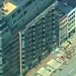
\includegraphics[width=0.13\linewidth]{img/case_1} &
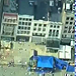
\includegraphics[width=0.13\linewidth]{img/case_2} &
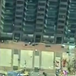
\includegraphics[width=0.13\linewidth]{img/case_3} &
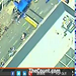
\includegraphics[width=0.13\linewidth]{img/case_4} \\
Ground Truth & 
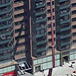
\includegraphics[width=0.13\linewidth]{img/case_1_grnd} &
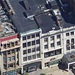
\includegraphics[width=0.13\linewidth]{img/case_2_grnd} &
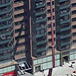
\includegraphics[width=0.13\linewidth]{img/case_3_grnd} &
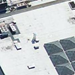
\includegraphics[width=0.13\linewidth]{img/case_4_grnd} \\
\hline
\multicolumn{5}{l}{\textbf{Ground Truth Ranking in All Database Images}} \\
\hline
VGG-CNN-M-$sim$ & 6 & 3 & 10 & 108\\
JSEM-$sim_R$ & 1 & 1 & 1 & 12\\
\end{tabular}
\caption{Case study on Boston Dataset.}
\label{table:bostoncase}
\end{table}

\begin{table*}[h]
\begin{tabular}{l|l|l|l|l|l|l|l|l|l}
\textbf{Model} & \textbf{N = 1} & \textbf{N = 2}& \textbf{N = 3}& \textbf{N = 4}& \textbf{N = 5}& \textbf{N = 10}& \textbf{N = 15} & \textbf{N = 20} & \textbf{N = 25} \\
\hline
VGG-CNN-M-$sim$ &7.05 & 13.85 & 21.41 & 25.44 & 30.23 & 44.33 & 51.89 & 62.97 & 69.77 \\
VGG-CNN-M-$sim_R$ & 8.31 & 15.87 & 23.43 & 30.23 & 35.52 & 53.40 & 73.05 & 80.35 & 84.13 \\
IBFT-$sim$ & 7.56 & 15.62 & 23.93 & 37.03 & 42.82 & 56.93 & 67.25 & 78.84 & 85.89 \\
JSEM-$sim_R$ & 16.12 & 27.96 & 39.80 & 51.39 & 58.44 & 78.84 & 84.63 & 89.67 & 95.21
\end{tabular}
\caption{Recall on top $N$ on Boston dataset.}
\label{table:boston_recall}
\end{table*} 


\begin{table*}[h]
\begin{tabular}{l|l|l|l|l|l|l|l|l|l}
\textbf{Model} & \textbf{N = 1} & \textbf{N = 2}& \textbf{N = 3}& \textbf{N = 4}& \textbf{N = 5}& \textbf{N = 10}& \textbf{N = 15} & \textbf{N = 20} & \textbf{N = 25} \\
\hline
VGG-CNN-M-$sim$ & 5.67&10.17& 14.42& 17.97& 20.33& 32.86& 46.57& 58.16& 68.32 \\
VGG-CNN-M-$sim_R$ & 5.91& 10.87& 15.84& 18.68& 21.04& 36.17& 47.28& 61.47& 70.92 \\
IBFT-$sim$ & 7.57& 11.58& 15.60& 18.91& 23.17& 34.04& 46.57& 55.79& 68.09 \\
JSEM-$sim_R$ & 9.22 & 15.60 & 21.28 & 25.77& 28.84&48.70&63.83&74.23&84.87 
\end{tabular}
\caption{Recall on Top $N$ on Tokyo TM dataset.}
\label{table:netvlad-result}
\end{table*} 

\begin{figure*}[h]
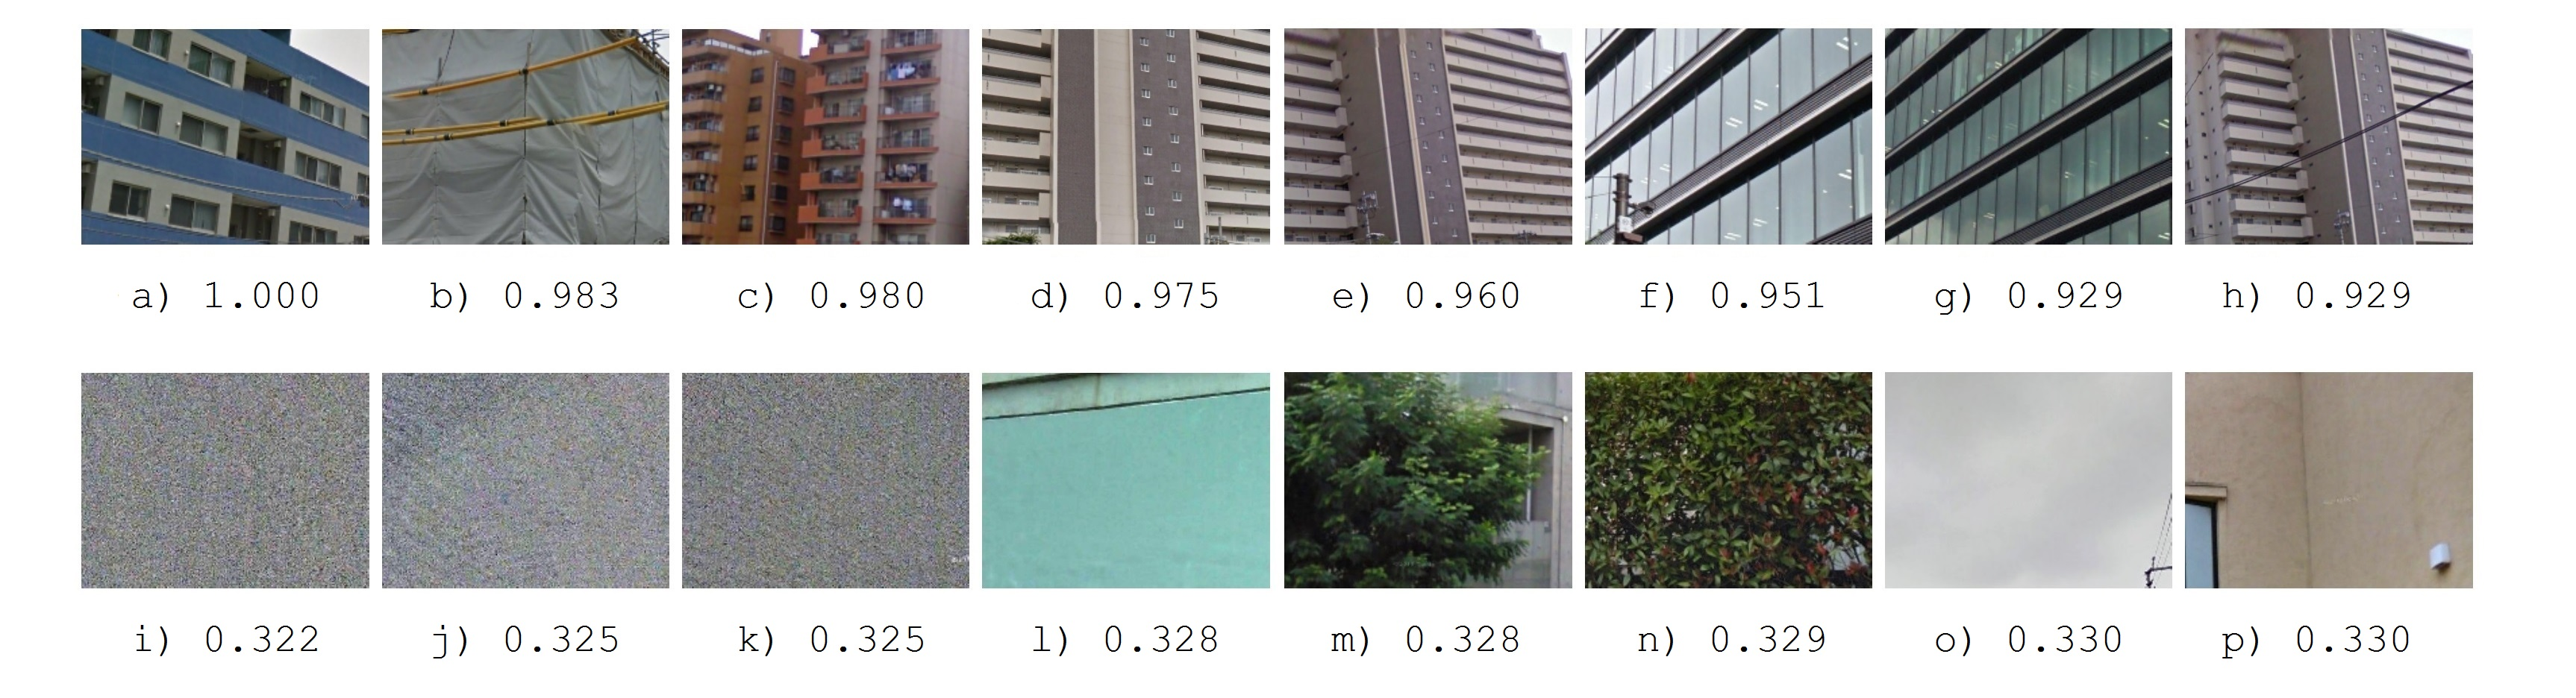
\includegraphics[width=0.9\textwidth]{img/salient}
\caption{8 most salient regions(top) and 8 most non-salient regions in Tokyo TM database, with their saliency score.}
\label{fig:saliency}
\end{figure*}

\emph{Boston: }
The result reported in Table~\ref{table:map} shows that our model has significantly improved the mean average precision (MAP) on the geo-localization task. For the convenience of view, Table~\ref{table:bostoncase} shows some case study on this task, from which we can easily see that the rankings of ground truth images raise a lot. In CNN, we resize the frames into a $224 \times 224$ square shape. Thus, we show the frames and database in such square shapes rather than rectangular ones in Figure~\ref{fig:bostonvideo}. Besides, the ``recall on top $K$'' result on Boston dataset is reported in Table~\ref{table:boston_recall}.

\emph{TokyoTM: }
We also run experiments on the Tokyo TM dataset and show results in Table~\ref{table:map} and Table~\ref{table:netvlad-result}. 

The experimental result had proved the efficiency of our model, showing that our model obtains the best recall for every $N$, and beats the baselines on the metric MAP. That is, our model not only performs well generally, but also has application value for real image retrieval tasks. However, it's interesting that the model IBFT-$sim$ performs  similar to VGG-CNN-M-$sim$ on Tokyo TM dataset. It suggests that fine-tuning based only on the limited training dataset could easily cause over-fitting. This also shows that saliency score is an important part to improve the performance of the model, and make the model more robust.

\subsection{Analysis of Learned Saliency}
To give further supporting evidences for the effectiveness of our method, we analyze the learned saliency qualitatively and quantitatively. 
We first conduct case study on some salient and non-salient regions, and then report the Pearson correlation with manually labeled saliency score on some randomly selected samples.

We applied the method introduced in Section~\ref{sec:solution} to estimate the saliency score for each region of a given image. 
Figure~\ref{fig:saliency} shows the 8 most salient and 8 most non-salient regions together with their saliency scores from the Tokyo TM database. 
The salient regions are all buildings with distinctive structure($a-h$) while the non-salient regions are images from road($i-k$), trees($m$ and $n$), sky($o$) and indistinctive building regions($l$ and $p$). 



We also analyze the correlation between learned saliency with saliency calculate from manually labeled building contour in manually-labeled-$sim_R$, which could be treated as ground truth saliency score. 
The Pearson correlation is $0.7625$, showing that our estimated saliency score has strong relation with the ground truth saliency score.
Figure~\ref{fig:saliencycasestudy} shows the case study of our region based saliency estimation on two specific images. 

\begin{figure}
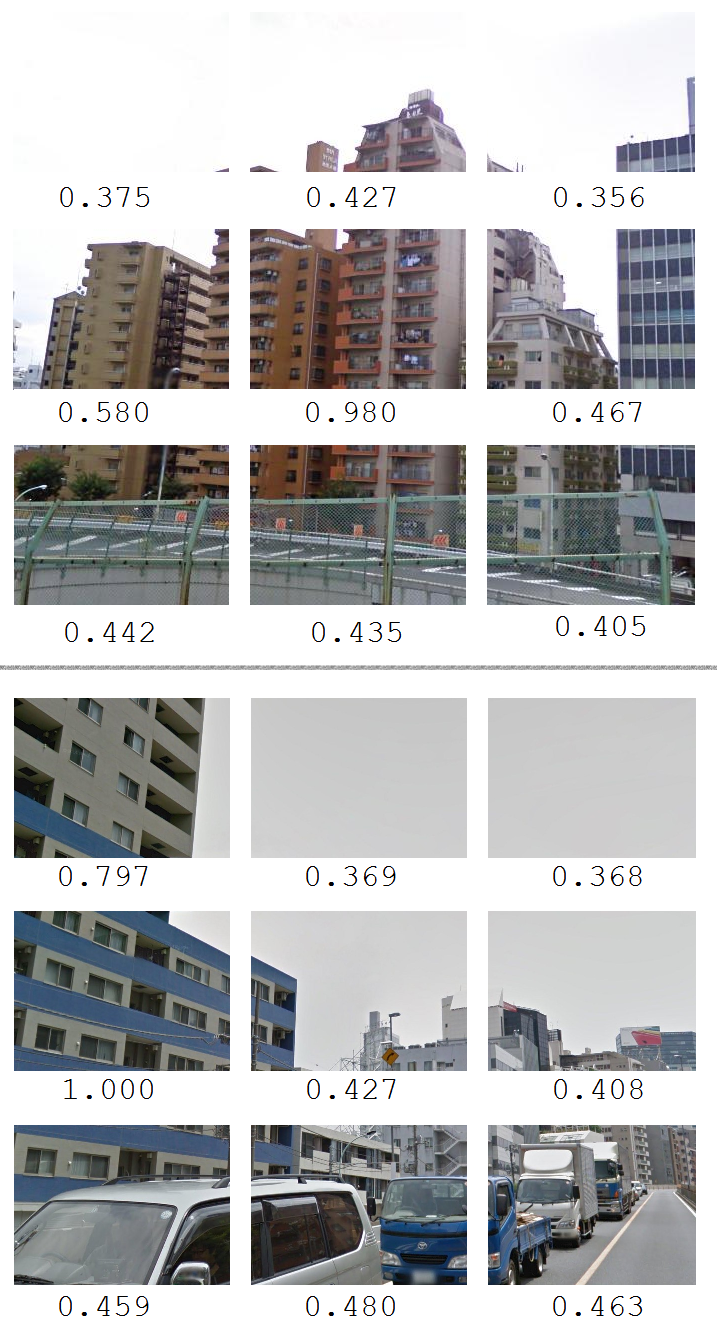
\includegraphics[width=0.73\linewidth]{img/case_study}
\caption{\label{fig:saliencycasestudy}Case study of region-based saliency estimation.}
\end{figure}
\section{Conclusions and Future Work}
\label{sec:conclusion}
We study automatic geo-localization of online event videos, which is the key component supporting various event analysis tasks such as cross camera tracking and 3d reconstruction. 
The major challenge lies in large appearance change of the environment due to human activity during the event. 
To solve this problem, we formulate the problem as region based joint saliency estimation and matching, and propose a solution, which iteratively estimates saliency and optimizes region based matching model.  
For the step of saliency optimization, we derived a closed form solution, which has an intuitive explanation. 
For region based matching model optimization, we apply self-paced learning algorithm to learn from the pseudo labels generated by saliency value estimated by matching. 
We conduct experiments on Boston Marathon 2013 dataset and Tokyo Time Machine datas	et to test the performance of our model. 
The experiments have shown that our solution significantly improves over matching on whole image and the automatically learned saliency has a strong correlation with manual labels on region saliency, proving that our model has significant application value. 
In the future, we will try more sophisticated CNN based models such as Resnet and NetVLAD in our matching model to improve performance.  
% As the cost of manually labeling all the exact matching point or region is unaffordable, weak labels are common situation in matching problems. 
% We will generalize this problem formulation to matching problems in different tasks at different levels: interest points and regions. 
% We also hope to design a framework based on current solution for a generalized problem formulation.


\newpage
\bibliographystyle{ACM-Reference-Format}
\bibliography{sigproc} 

\end{document}
